% Author: Izaak Neutelings (Februari, 2020)

\documentclass[border=3pt,tikz]{standalone}
\usepackage{amsmath} % for \dfrac
\usepackage{physics,siunitx}
\usepackage{tikz,pgfplots}
\usetikzlibrary{angles,quotes} % for pic (angle labels)
\usetikzlibrary{decorations.markings}
\tikzset{>=latex} % for LaTeX arrow head
\usepackage{xcolor}
\colorlet{Rcol}{green!60!black}
\colorlet{myblue}{blue!70!black}
\colorlet{myred}{red!70!black}
\colorlet{Ecol}{orange!90!black}
\tikzstyle{Rline}=[Rcol,thick]
\tikzstyle{gline}=[Rcol,thick]
\tikzstyle{bline}=[myblue,thick]
\tikzstyle{rline}=[myred,thick]
\def\xmax{4.5}
\def\ymax{3}
\def\tick#1#2{\draw[thick] (#1) ++ (#2:0.03*\ymax) --++ (#2-180:0.06*\ymax)}
\newcommand\EMF{\mathcal{E}} %\varepsilon}


\begin{document}


% OHMIC RESISTORS
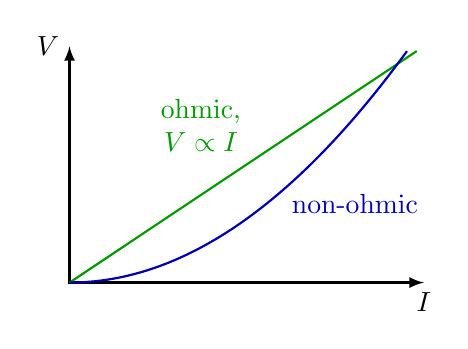
\begin{tikzpicture}
  \def\a{0.16}
  \coordinate (O) at (0,0);
  \coordinate (X) at (\xmax,0);
  \coordinate (Y) at (0,\ymax);
  
  % AXIS
  \draw[<->,thick]
    (X) node[below] {$I$} -- (O) -- (Y) node[left] {$V$};
  
  % PLOT
  \draw[Rline,samples=100,smooth,variable=\x,domain=0:0.98*\xmax]
    plot(\x,\ymax/\xmax*\x);
  \draw[bline,samples=100,smooth,variable=\x,domain=0:{sqrt(0.98*\ymax/\a)}]
    plot(\x,\a*\x^2);
  \node[Rcol,left,align=center] at (2.3,2.0) {ohmic,\\$V \propto I$};
  \node[myblue,right] at (2.7,1.0) {non-ohmic};
  
\end{tikzpicture}


% RESISTIVITY
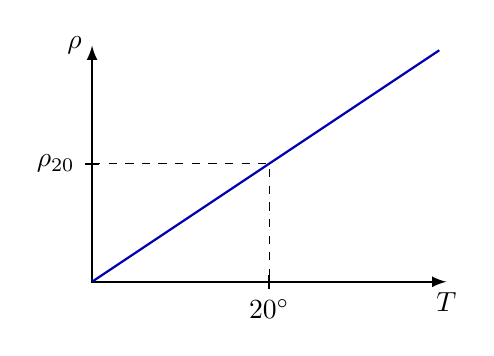
\begin{tikzpicture}
  \def\a{\ymax/\xmax}
  \def\Tz{0.5*\xmax}
  \coordinate (O) at (0,0);
  \coordinate (X) at (\xmax,0);
  \coordinate (Y) at (0,\ymax);
  \coordinate (P) at (\Tz,\a*\Tz);
  \coordinate (Px) at (\Tz,0);
  \coordinate (Py) at (0,\a*\Tz);
  
  % AXIS
  \draw[<->,thick]
    (X) node[below] {$T$} -- (O) -- (Y) node[left] {$\rho$};
  \tick{Px}{90} node[below] {$\SI{20}{\degree}$};
  \tick{Py}{ 0} node[left] {$\rho_{20}$};
  
  % PLOT
  \draw[bline,samples=100,smooth,variable=\x,domain=0:0.98*\xmax]
    plot(\x,\a*\x);
  \draw[dashed] (Py) -- (P) -- (Px);
  %\node[above right] at (1.4,1.8) {$E \sim \dfrac{1}{T}$};
  
\end{tikzpicture}


% RESISTIVITY
\begin{tikzpicture}
  \def\a{2.4}
  \coordinate (O) at (0,0);
  \coordinate (X) at (\xmax,0);
  \coordinate (Y) at (0,\ymax);
  
  % AXIS
  \draw[<->,thick]
    (X) node[below] {$T$} -- (O) -- (Y) node[left] {$\rho$};
  
  % PLOT
  \draw[bline,samples=100,smooth,variable=\x,domain={1.1*\a/\ymax}:0.98*\xmax]
    plot(\x,\a/\x);
  %\node[above right] at (1.4,1.8) {$E \sim \dfrac{1}{T}$};
  
\end{tikzpicture}


% RESISTIVITY
\begin{tikzpicture}
  \def\a{0.25}
  \def\Tc{1.8}
  \def\rc{0.35*\ymax}
  \coordinate (O) at (0,0);
  \coordinate (X) at (\xmax,0);
  \coordinate (Y) at (0,\ymax);
  \coordinate (P) at (\Tc,\rc);
  \coordinate (Px) at (\Tc,0);
  \coordinate (Py) at (0,\rc);
  
  % AXIS
  \draw[<->,thick]
    (X) node[below] {$T$} -- (O) -- (Y) node[left] {$\rho$};
  %\tick{Py}{ 0} node[below=-1,left] {$\dfrac{kQ}{R^2}$};
  \tick{Px}{90} node[below] {$T_\mathrm{c}$};
  
  % PLOT
  \draw[bline,samples=100,smooth,variable=\x,domain=\Tc:{sqrt((0.98*\ymax-\rc)/\a))+\Tc}]
    plot(\x,{\rc+\a*(\x-\Tc)^2});
  \draw[bline]
    (0,0.005*\ymax) --++ (Px);
  %\node[above right] at (2.8,1.6) {$E \sim \dfrac{1}{r^2}$};
  \draw[dashed]
    (Py) -- (P) -- (Px);
  
\end{tikzpicture}


% RC circuit Q decharging
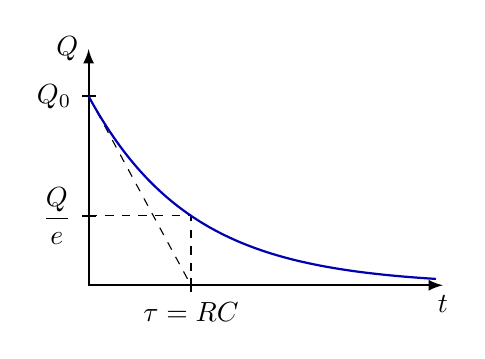
\begin{tikzpicture}
  \def\a{2.4}
  \def\t{1.3}
  \coordinate (O) at (0,0);
  \coordinate (X) at (\xmax,0);
  \coordinate (Y) at (0,\ymax);
  \coordinate (Q) at (0,\a);
  \coordinate (T) at (\t,\a/2.718);
  \coordinate (Tx) at (\t,0);
  \coordinate (Ty) at (0,\a/2.718);
  
  % AXIS
  \draw[<->,thick]
    (X) node[below] {$t$} -- (O) -- (Y) node[left] {$Q$};
  \tick{Q}{0} node[left] {$Q_0$};
  \tick{Tx}{90} node[below] {$\tau = RC$};
  \tick{Ty}{0} node[left] {$\dfrac{Q}{e}$};
  
  % PLOT
  \draw[dashed] (Q) -- (Tx);
  \draw[dashed] (Ty) -- (T) -- (Tx);
  \draw[bline,samples=100,smooth,variable=\x,domain=0:0.98*\xmax]
    plot(\x,{\a*exp(-\x/\t)});
  
\end{tikzpicture}


% RC circuit Q charging
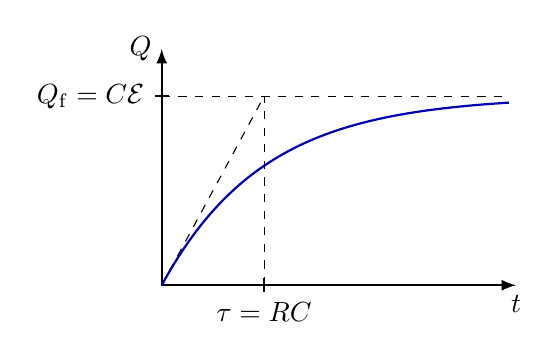
\begin{tikzpicture}
  \def\a{2.4}
  \def\t{1.3}
  \coordinate (O) at (0,0);
  \coordinate (X) at (\xmax,0);
  \coordinate (Y) at (0,\ymax);
  \coordinate (Q) at (0,\a);
  \coordinate (T) at (\t,\a);
  \coordinate (Tx) at (\t,0);
  
  % AXIS
  \draw[<->,thick]
    (X) node[below] {$t$} -- (O) -- (Y) node[left] {$Q$};
  \tick{Q}{0} node[left] {$Q_\mathrm{f} = C\EMF$};
  \tick{Tx}{90} node[below] {$\tau = RC$};
  
  % PLOT
  \draw[dashed] (Q) --++ (0.98*\xmax,0);
  \draw[dashed] (Tx) -- (T);
  \draw[dashed] (O) -- (T);
  \draw[bline,samples=100,smooth,variable=\x,domain=0:0.98*\xmax]
    plot(\x,{\a*(1-exp(-\x/\t)});
  
\end{tikzpicture}


% RC circuit I charging
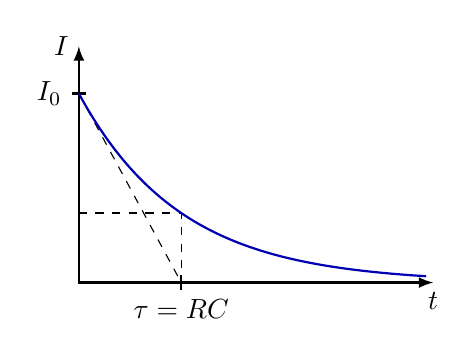
\begin{tikzpicture}
  \def\a{2.4}
  \def\t{1.3}
  \coordinate (O) at (0,0);
  \coordinate (X) at (\xmax,0);
  \coordinate (Y) at (0,\ymax);
  \coordinate (I) at (0,\a);
  \coordinate (T) at (\t,\a/2.718);
  \coordinate (Tx) at (\t,0);
  \coordinate (Ty) at (0,\a/2.718);
  
  % AXIS
  \draw[<->,thick]
    (X) node[below] {$t$} -- (O) -- (Y) node[left] {$I$};
  \tick{I}{0} node[left] {$I_0$};
  \tick{Tx}{90} node[below] {$\tau = RC$};
  
  % PLOT
  \draw[dashed] (I) -- (Tx);
  \draw[dashed] (Ty) -- (T) -- (Tx);
  \draw[bline,samples=100,smooth,variable=\x,domain=0:0.98*\xmax]
    plot(\x,{\a*exp(-\x/\t)});
  
\end{tikzpicture}


% RCL circuit I charging
\begin{tikzpicture}
  \def\a{2.4}
  \def\t{1.3}
  \coordinate (O) at (0,0);
  \coordinate (X) at (\xmax,0);
  \coordinate (Y) at (0,\ymax);
  \coordinate (I) at (0,\a);
  \coordinate (T) at (\t,\a);
  \coordinate (Tx) at (\t,0);
  
  % AXIS
  \draw[<->,thick]
    (X) node[below] {$t$} -- (O) -- (Y) node[left] {$I$};
  \tick{Q}{0} node[left] {$I_\mathrm{f} = \dfrac{\EMF_0}{R}$};
  \tick{Tx}{90} node[below] {$\tau = L/R$};
  
  % PLOT
  \draw[dashed] (I) --++ (0.98*\xmax,0);
  \draw[dashed] (Tx) -- (T);
  \draw[dashed] (O) -- (T);
  \draw[bline,samples=100,smooth,variable=\x,domain=0:0.98*\xmax]
    plot(\x,{\a*(1-exp(-\x/\t)});
  
\end{tikzpicture}


% RC circuit I discharging
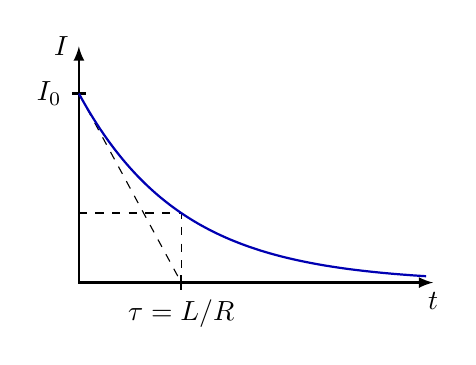
\begin{tikzpicture}
  \def\a{2.4}
  \def\t{1.3}
  \coordinate (O) at (0,0);
  \coordinate (X) at (\xmax,0);
  \coordinate (Y) at (0,\ymax);
  \coordinate (I) at (0,\a);
  \coordinate (T) at (\t,\a/2.718);
  \coordinate (Tx) at (\t,0);
  \coordinate (Ty) at (0,\a/2.718);
  
  % AXIS
  \draw[<->,thick]
    (X) node[below] {$t$} -- (O) -- (Y) node[left] {$I$};
  \tick{I}{0} node[left] {$I_0$};
  \tick{Tx}{90} node[below] {$\tau = L/R$};
  
  % PLOT
  \draw[dashed] (I) -- (Tx);
  \draw[dashed] (Ty) -- (T) -- (Tx);
  \draw[bline,samples=100,smooth,variable=\x,domain=0:0.98*\xmax]
    plot(\x,{\a*exp(-\x/\t)});
  
\end{tikzpicture}


% RCL circuit V, Q alternating
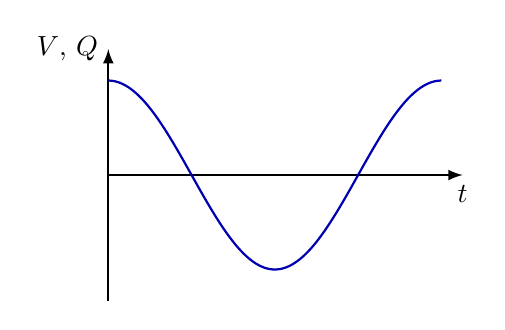
\begin{tikzpicture}
  %\def\xmax{9}
  \def\ymax{1.6}
  \def\a{1.2}
  \def\t{360/(0.94*\xmax)}
  \coordinate (O) at (0,0);
  \coordinate (X) at (\xmax,0);
  \coordinate (Y) at (0,\ymax);
  
  % AXIS
  \draw[->,thick]
    (0,-\ymax) -- (Y) node[left] {$V$, $Q$};
  \draw[->,thick]
    (O) -- (X) node[below] {$t$};
  
  % PLOT
  \draw[bline,samples=100,smooth,variable=\x,domain=0:0.94*\xmax]
    plot(\x,{\a*cos(\t*\x)});
  
\end{tikzpicture}


% RCL circuit I alternating
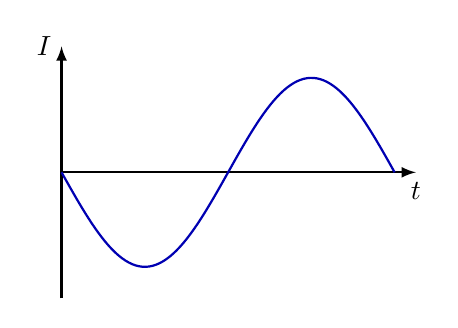
\begin{tikzpicture}
  %\def\xmax{9}
  \def\ymax{1.6}
  \def\a{1.2}
  \def\t{360/(0.94*\xmax)}
  \coordinate (O) at (0,0);
  \coordinate (X) at (\xmax,0);
  \coordinate (Y) at (0,\ymax);
  
  % AXIS
  \draw[->,thick]
    (0,-\ymax) -- (Y) node[left] {$I$};
  \draw[->,thick]
    (O) -- (X) node[below] {$t$};
  
  % PLOT
  \draw[bline,samples=100,smooth,variable=\x,domain=0:0.94*\xmax]
    plot(\x,{-\a*sin(\t*\x)});
  
\end{tikzpicture}


% RCL circuit Q alternating, exponential
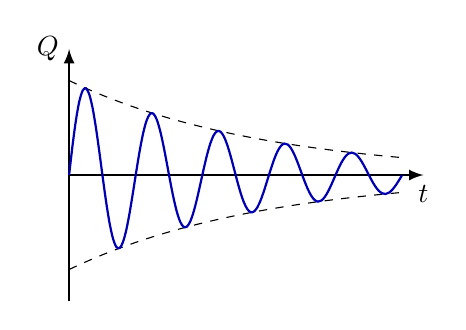
\begin{tikzpicture}
  %\def\xmax{9}
  \def\ymax{1.6}
  \def\a{1.2}
  \def\t{1800/(0.94*\xmax)}
  \def\T{0.4}
  \coordinate (O) at (0,0);
  \coordinate (X) at (\xmax,0);
  \coordinate (Y) at (0,\ymax);
  
  % AXIS
  \draw[->,thick]
    (0,-\ymax) -- (Y) node[left] {$Q$};
  \draw[->,thick]
    (O) -- (X) node[below] {$t$};
  
  % PLOT
  \draw[dashed,samples=100,smooth,variable=\x,domain=0:0.94*\xmax]
    plot(\x,{\a*exp(-\T*\x)}) plot(\x,{-\a*exp(-\T*\x)});
  \draw[bline,samples=100,smooth,variable=\x,domain=0:0.94*\xmax]
    plot(\x,{\a*exp(-\T*\x)*sin(\t*\x)});
  
\end{tikzpicture}



\end{document}
